\section{Problems}

\frame{
With used amplifiers, the following oscillations at the amplifier output with DC power can be observed:

\begin{center}
    \incfig{scheme5}
\end{center}

This is due to the instability of the amplifier. 
% This instability can be eliminated by the adjustment of the scheme. 

\phantom{42}

The main problem is that desired oscillations $\sim 10$ ns. \\

\phantom{42}

We proceeded to experiments with faster amplifiers, but it is usefull to understand results of such delays.

oscillations megahertz
 \frametitle{Problems}}

% \frame{
% However, it was not possible to move to the chaotic regime in the laser. Possible cause of the problem may be
\begin{itemize}
    \iitem{parasitic capacity and inductance,}
\end{itemize}
In terms of solutions -- neatly soldered scheme.


% \phantom{42}

% A suitable amplifier, with similar properties used in the article, must come in June. \frametitle{Problems}}


\frame{
In real system\footnote{
    S. Tang, J. M. Liu, <<Chaotic pulsing and quasi-periodic route to chaos in a semiconductor laser with delayed opto-electronic feedback>>, 2001.
}  $S_0^{-1} \int_{0}^{\infty} f(\eta) S(t-\eta)d\eta$ instead of $S(t-\tau)$. \\
 It reduces oscillations.
 \frametitle{Real system}}



\section{Results}

% добаввить 2 слайда:
% успехи численного моедлирования
    % показали, что хаос есть
    % численно нашли ограничения
    % про это не говорилось в статье
% успехи реализация
    % разработали схему
    % пос
    % стабильные оу
% ключевые ограничения:
    % 

% 



\frame{
Modeled good numerical solution. The existence of chaos is shown. The maximum <<slowness>> of the system is estimated.

\begin{minipage}[b]{0.49\textwidth}
      \begin{figure}[h]
          \centering
          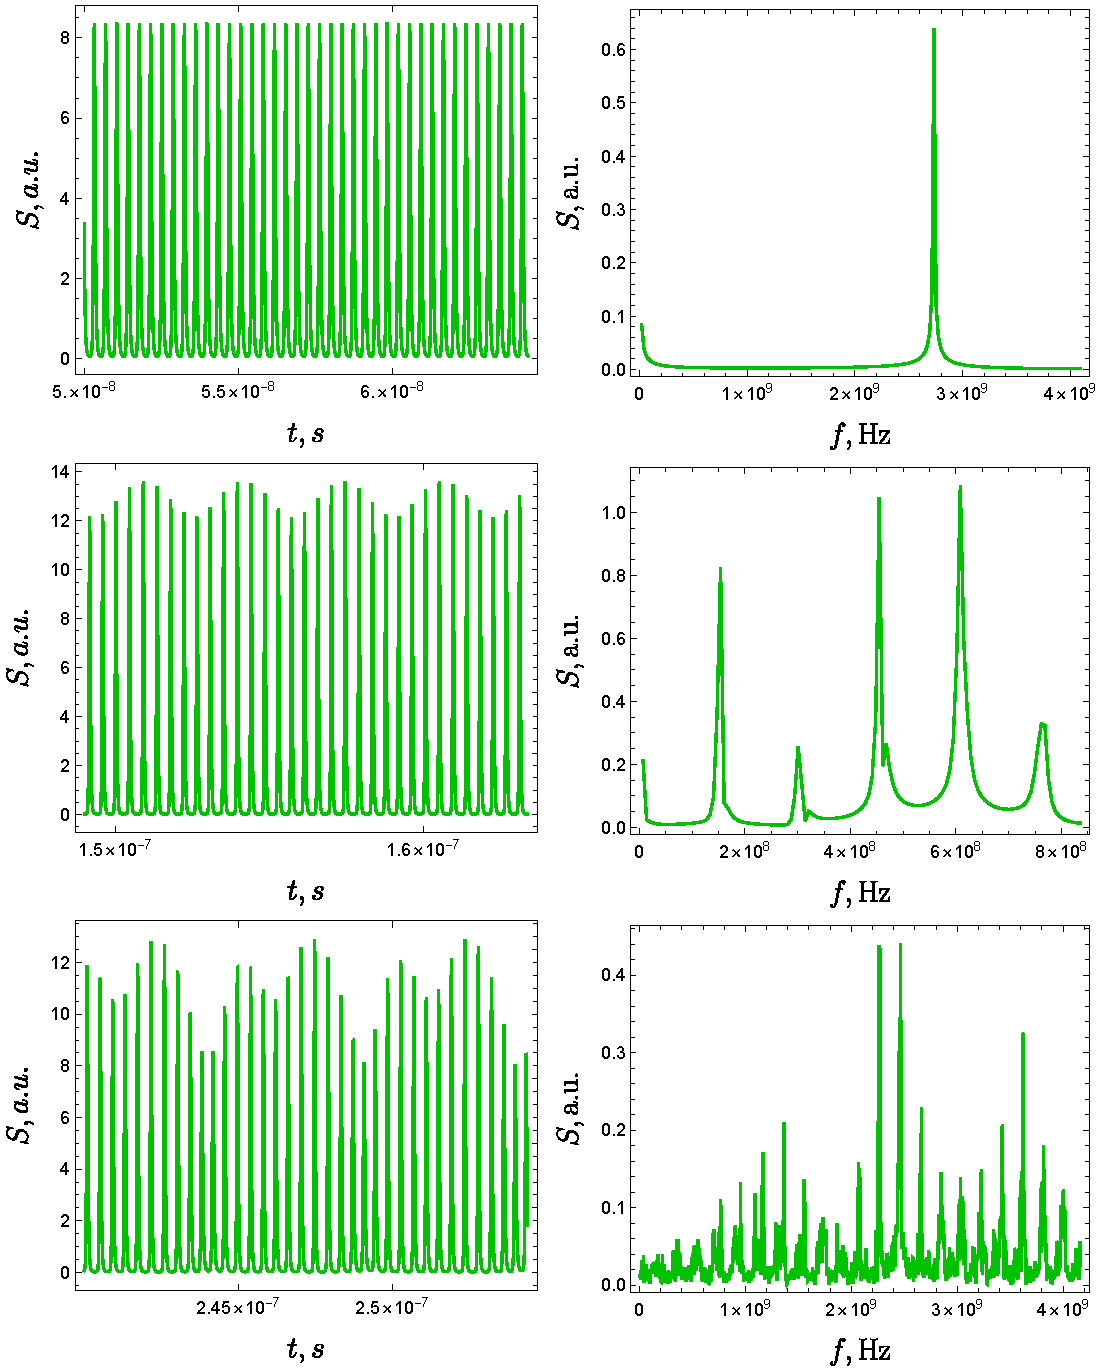
\includegraphics[width=0.85\textwidth]{figures/modeling_vertical.pdf}
          \caption{Modeling}
      \end{figure}
\end{minipage}
\hfill
\begin{minipage}[b]{0.49\textwidth}
    \begin{figure}[h]
    \centering
    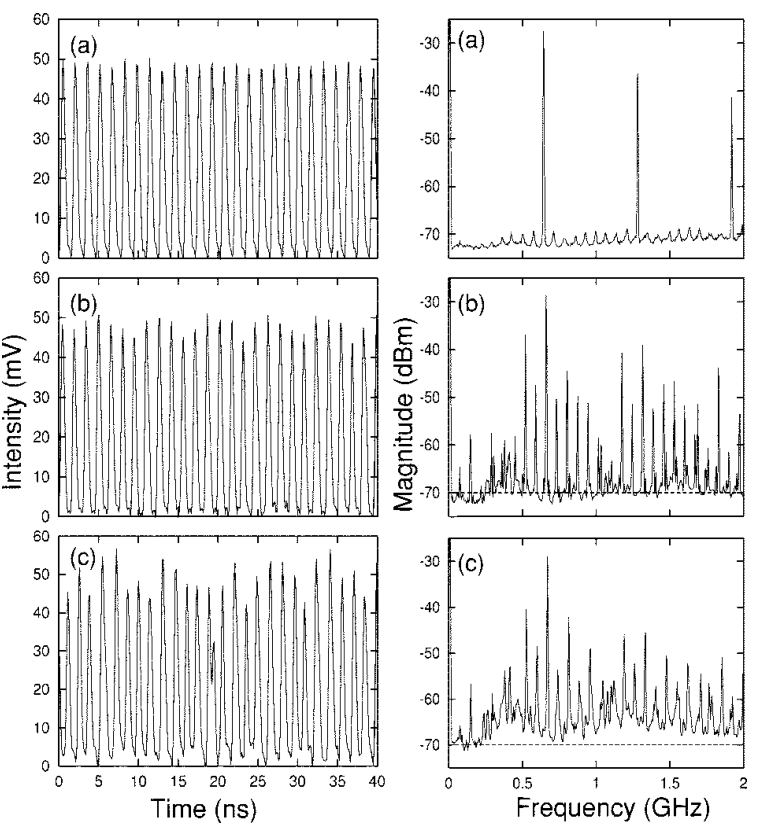
\includegraphics[width=0.85\textwidth]{images/tang_exp.png}
    \caption{Article experiment}
    %\label{fig:}
    \end{figure}
\end{minipage}

 \frametitle{Results in the modeling}}

\frame{
Principal restrictions in implementation:
\begin{itemize}
    \iitem{High-frequency oscillations,
        so, as we found, equipment for working at a frequency $\geq  (10 \tau_\text{r})^{-1} \approx 200$ MGz is necessary.
    }
    \iitem{No possibility for a specific laser change the frequency of oscillations.}
\end{itemize}


Successes on the way to implementation:
\begin{itemize}
    \iitem{Optimal values for $\tau_\text{delay}$ and laser range were found selected; stabilized operational amplifiers;}
    \iitem{A scheme has been developed, a slow positive feedback is implemented.}
    \iitem{A video signal transmission system is adjusted, also ovserved the constant behavior
    with $\tau_{\text{i}} \approx 50 \tau_{\text{r}}$
    .}
\end{itemize}

 \frametitle{Results in the practice work}}


\frame{
As a result of the project:
\begin{itemize}
    \iitem{According to the equations of the laser's evolution with a feedback, the \textbf{numerical model was built} in the ideal and non ideal case.}
    \iitem{It is shown that \textbf{chaos is possible in the system}. Chaos parameters are estimated. The frequency limitation were evaluated for the system. }
    \iitem{A scheme of positive feedback has been developed and built. The optimal parameters for the scheme were selected.}
    \iitem{Got prepared for the use of an industrial setup.}
\end{itemize}

 \frametitle{Сonclusion}}



